\section*{Ejercicio 3}

¿Las siguientes transformaciones son inyectivas, suprayectivas o ambas?








\begin{enumerate}
%%%%%%%%%%%%%%%%%%%%%%%%%%%%%%%%%
%%%%%%%%%%%%%%%%%%%%%%%%%%%%%%%%%
%%%%% EJERCICIO 3.B      
    \item $T: \R^{2} \rightarrow \R^{3}$ tal que $T(a,b) = (a + b, 0, 2a - b)$
%%%%%%%%%%%%%%%%%%%%%%%%%%%%%%%%%

      Recordando el teorema 1.22 (Sean V y W espacios vectoriales sobre un campo F. Sea \(T:V \to W\) una transformación
       lineal. Entonces, \(T\) es inyectiva si y solo si \(\text{Ker}(T)=\{0v\}\).) Por lo cual calcularemos el núcleo
       de \(T\).\\

      El núcleo de \(T\) es el conjunto de todos los vectores \((a, b)\) en \(\mathbb{R}^2\) que se mapean a
       \((0, 0, 0)\) en \(\mathbb{R}^3\). En otras palabras, necesitamos encontrar todas las soluciones de la ecuación
       \(T(a,b) = (0, 0, 0)\). \\
       
      La transformación \(T\) se define como: \(T(a,b) = (a+b, 0, 2a-b)\) y para encontrar el
       núcleo resolveremos \(T(a,b) = (0, 0, 0)\). Lo que nos da el siguiente sistema de ecuaciones:
      \begin{center}      
      \begin{minipage}{2cm}
            \begin{align*}
                  a + b = 0 & \\
                  0 = 0 & \rightarrow \\
                  2a - b = 0 &
            \end{align*}
      \end{minipage}
      \begin{minipage}{3cm}
            \begin{align*}
                  a + b = 0 &  \\                  
                  2a - b = 0 &
            \end{align*}
      \end{minipage}
      \end{center}

      Lo que nos da 
      \begin{align*}
            b = & -a \\
            2a -(-a) = 0 \rightarrow 3a = 0 \rightarrow a = &  0 \\
            b = & 0
      \end{align*}

      Esto significa que la única solución al sistema \(T(a,b) = (0,0,0)\) es \((a,b) = (0,0)\). En otras palabras, el núcleo de \(T\) consiste únicamente en el vector nulo \((0,0)\).

      Dado que el núcleo de \(T\) es igual al conjunto nulo, hemos demostrado que \(T\) es inyectiva según el teorema anteriormente citado, ya que no hay ningún otro par de vectores \((a,b)\) que se mapee a \((0,0,0)\) aparte del vector nulo.

      Una transformación lineal es sobreyectiva si la imagen de la transformación abarca todo el espacio de destino. Esto significa que, para cualquier vector \((x, y, z)\) en \(\mathbb{R}^3\), debe haber un vector \((a, b)\) en \(\mathbb{R}^2\) tal que \(T(a, b) = (x, y, z)\).

      Tomemos un vector genérico \((x, y, z)\) en \(\mathbb{R}^3\). Queremos encontrar valores de \(a\) y \(b\) que hagan que \(T(a, b) = (x, y, z)\), es decir:

      \begin{align*}
            a + b & \, = x \\
                0 & \, = y \\
            2a - b& \, = z \\
      \end{align*}

      Dado que $0 = y$, sabemos que $y$ debe ser igual a 0. Esto implica las ecuaciones:
      \begin{align*}
            a + b & \, = x \\
            2a - b& \, = z \\
      \end{align*}

      Y resolvemos el sistema de ecuaciones:
      \begin{equation*}
            a + b = x \rightarrow b = x - a
      \end{equation*}
      \begin{align*}
            2a - b & \, = \, z \\
            2a - (x - a) & \, = \, z \\
            3a - x & \, = \, z \\
            3a  & \, = \, z + x \\
            a & \, = \, \frac{z + x}{3} \\
      \end{align*}
      \begin{equation*}
            b = x - a \rightarrow b = x - \frac{z+x}{3}
      \end{equation*}

      Entonces, hemos encontrado una expresión para \(a\) y \(b\) en términos de \(x\) y \(z\). Por lo tanto,
       para cualquier vector \((x, y, z)\) en \(\mathbb{R}^3\), podemos encontrar un vector \((a, b)\) en
       \(\mathbb{R}^2\) tal que \(T(a, b) = (x, y, z)\). Esto demuestra que \(T\) es una transformación sobreyectiva.

      \begin{center}
            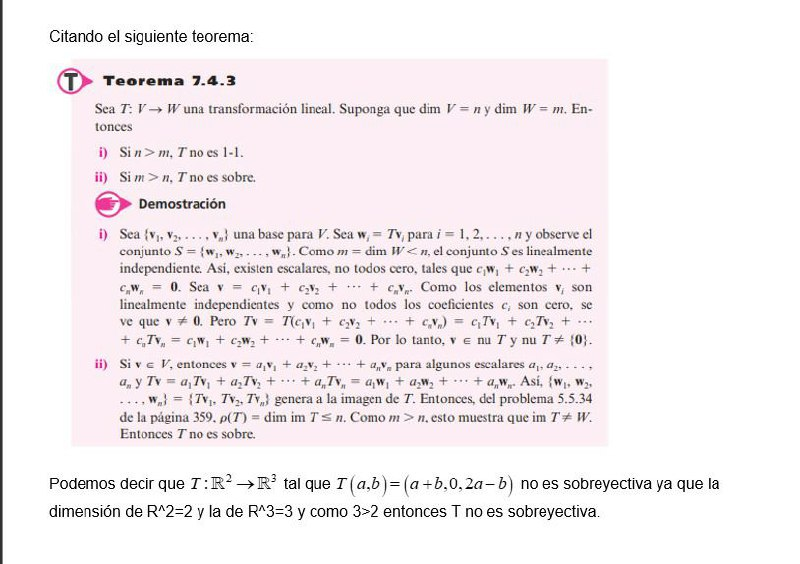
\includegraphics[scale = .5]{IMA/teorema2.jpg}
      \end{center}






%%%%%%%%%%%%%%%%%%%%%%%%%%%%%%%%%
%%%%%%%%%%%%%%%%%%%%%%%%%%%%%%%%%
%%%%% EJERCICIO 3.B
    \item $T: \R^{5} \rightarrow \R^{5}$ tal que $T(a,b,c,d,e)  = (a + 2b -c, -3a + b + 4c, a - b + 2d, b + c +3e, 2a + b + d - e)$\\
%%%%%%%%%%%%%%%%%%%%%%%%%%%%%%%%%


      Para demostrar que la transformación lineal $T: \R^{5} \rightarrow \R^{5}$ es inyectiva, debemos demostrar
      que el núcleo (kernel) de $T$ es el vector nulo (0,0,0,0,0). Esto significa que si $T(a,b,c,d,e) = T(x,y,z,w,v)$,
      entonces $a = x, b = y, c = z, d = w, e = v$. En otras palabras $T(a,b,c,d,e) = T(x,y,z,w,v)$ implica que 
      $(a,b,c,d,e) = (x,y,z,w,v)$\\

      La transformación lineal $T$ se define como:

      \begin{equation*}
            T(a,b,c,d,e)  = (a + 2b -c, -3a + b + 4c, a - b + 2d, b + c +3e, 2a + b + d - e)
      \end{equation*}

      Para demostrar la inyectividad, supongamos que $T(a,b,c,d,e) = T(x,y,z,w,v)$, lo que significa que:

      \begin{equation*}
            (a + 2b -c, -3a + b + 4c, a - b + 2d, b + c + 3e, 2a + b + d - e) = T(x,y,z,w,v) 
      \end{equation*}

      Esto nos lleva a un sistema de ecuaciones lineales: 
      \begin{equation}
            a + 2b -c = x \tag{3.1} \label{ec3.1}
      \end{equation}
      \begin{equation*}
            -3a + b + 4c = y \tag{3.2} \label{ec3.2}
      \end{equation*}
      \begin{equation}
            a - b + 2d = z \tag{3.3} \label{ec3.3}
      \end{equation}
      \begin{equation}
            b + c + 3e = w \tag{3.4} \label{ec3.4}
      \end{equation}
      \begin{equation}
            2a + b + d - e = v \tag{3.5} \label{ec3.5} 
      \end{equation}

      Queremos demostrar que la única solución para este sistema es $(a,b,c,d,e) = (x,y,z,w,v)$. Para
      hacerlo, podemos utilizar álgebra lineal y métodos de resolución de sistemas de ecuaciones

      Conocemos la primera ecuación \eqref{ec3.1}
            
      Restamos la primera ecuación \eqref{ec3.1} de la segunda \eqref{ec3.2}

      \begin{equation*}
            (-3a + b + 4c) - (a + 2b -c) = y -x
      \end{equation*}
      
      Simplificamos 
      \begin{equation*}
            -2a - b + 5c = y - x
      \end{equation*}
      
      Despejamos $a$
      \begin{equation*}
            a = \frac{y-x+b+5c}{-2}
      \end{equation*}
      Ahora, utilicemos esta expresión para $a$ en la tercera ecuación \eqref{ec3.3}
      \begin{equation*}
            \left( \frac{y-x+b+5c}{(-2)}   \right)  - b + 2d = z
      \end{equation*}
      Simplifiquemos:
      \begin{equation*}
            (-y + x -b - 5c) -3b +4d = 2z
      \end{equation*}
      Despejamos $b$
      \begin{equation*}
            b = \frac{x-y-5c-2z}{3} + 2d
      \end{equation*}
      Ahora sustituyamos esta expresión para $b$ en la cuarta ecuación \eqref{ec3.4}
      \begin{equation*}
            \left( \frac{x - y - 5c  - 2}{3} \right) + c  + 3e = w
      \end{equation*}
      Simplificamos
      \begin{equation*}
            \frac{x-y-2z}{3} + 2d +4c +3e = w
      \end{equation*}
      Despejamos $c$ 
      \begin{equation*}
            c = \frac{(3w - x + y 2z - 6d -9e)}{4}
      \end{equation*}
      Finalmente, utilicemos estas expresiones para $a$, $b$ y $c$ en la quinta ecuación \eqref{ec3.5}
      \begin{equation*}
            2 \left(\frac{y-x+b+5c}{2}\right) + \left(\frac{x-y-5c-2z}{3+2d-e}\right) = v
      \end{equation*}
      Simplifiquemos
      \begin{align*}
            -(y-x+b+5c) + \frac{x-y-5c -2z}{3 + 2d -e} & \,\, = v \\
            -\left(y-x+ (\frac{x-y-5c-2z}{3}) + 5c\right) + 2d -3 & \,\, = v  \\
            -\left(y-x+\frac{x}{3} - \frac{y}{3} - \frac{5c}{3} - \frac{2z}{3} + 5c\right) + 2d -e & \,\, = v \\
            -\frac{2y}{3} + \frac{2x}{3} -\frac{7c}{3} - \frac{2z}{3}  + 2d - e & \,\, = v \\
            \frac{(2x -2y -7c -2z +6d -3e)}{3} & \,\, = v
      \end{align*}
      De esta ecuación, podemos despejar $e$
      \begin{equation*}
            e = \frac{(2x - 2y -7c - 2z +6d -3v)}{3}
      \end{equation*}

      Hemos expresado todas las variables $a,b,c,d,e$ en términos de $(x.y,z,w,v)$. Esto demuestra que para cualquier 
      conjunto de valores $(x.y,z,w,v)$ en $\R^{5}$ existe un conjunto correspondiente de valores $(a,b,c,d,e)$ en $\R^{5}$
      que satisface el sistema de ecuaciones. $\therefore$ Hemos demostrado que $T$ es inyectiva.

      Sabemos que $dim(\R^{5}) = 5$ y además $T$ es inyectiva, por lo que por el teorema $1.25$ podemos decir que $T$ también es Sobreyectiva.
      \begin{center}
            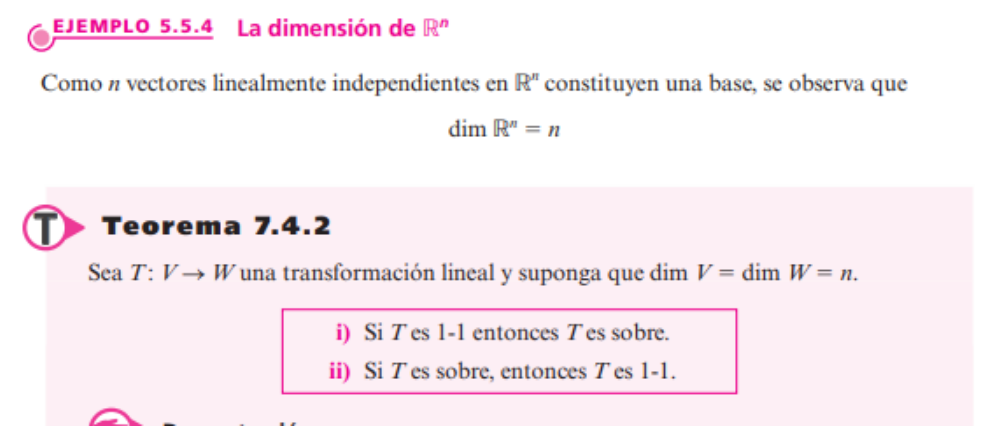
\includegraphics[scale = .6]{IMA/teorema 7.4.2.png}
      \end{center}

      \textbf{Teorema 1.22} Sean $V$ y $W$ espacios vectoriales sobre un campo $F$. Sea $T: V \rightarrow W$ una
      transformación lineal. Entonces, $T$ es inyectiva si y solo si $Ker(T) = \{ 0_{V}\}$ \\

      \textbf{Teorema 1.23} Sean $V$ y $W$ espacio vectoriales sobre un campo $F$. Sea $T: V \rightarrow W$ una
      transformación lineal. Las siguientes condiciones son equivalentes:
      \begin{enumerate}
            \item[1.] $T$ es inyectiva;
            \item[2.] Para cualquier subconjunto $S \subseteq V$, se tiene que $S$ es linealmente independiente en $V$ si y solo si $T(S) := \{ T(s) : s \in S\}$
                  es linealmente independiente en $W$
            
      \end{enumerate}

      $\textbf{\text{Teorema 1.25}}^{\textcolor{red}{7}}$ Sean $V$ y $W$ espacios vectoriales de dimensión finita  sobre un campo $F$ con $dim_{F}(V) = dim_{F}(W).$
      Sea $T: V \rightarrow W$ una transformación lineal. Los siguientes enunciados son equivalentes.
      \begin{enumerate}
            \item[1.] $T$ es inyectiva
            \item[2.] $T$ es suprayectiva
            \item[3.] $T$ es biyectiva
      \end{enumerate}
      

      
      
\end{enumerate}























